\documentclass{article}

\usepackage[utf8]{inputenc}
\usepackage[T1]{fontenc}
\usepackage{lipsum}
\usepackage{graphicx}
\usepackage{amsmath}
\usepackage[margin=1in]{geometry}
\usepackage{titlesec}
\usepackage{enumitem}

\titleformat{\section}
{\LARGE\bfseries}{\thesection}{1em}{}

\titleformat{\subsection}
{\Large\bfseries}{\thesection}{1em}{}

\begin{document}
\pagestyle{empty}
\section*{Software testing}
\large

\subsection*{Introduzione}
\large
Obiettivi:
\begin{itemize}
    \renewcommand{\labelitemi}{-}
    \itemsep0em
    \item Comprendere l'importanza del software testing all'interno delle fasi di sviluppo del sistema
    \item Adeguare propriamente metodiche di testing affinchè sia acquisibile un certo livello di confidenza con il sistema software elaborato
\end{itemize}
Parte cruciale all'interno di un qualsiasi processo di sviluppo software consiste nella creazione di \textit{testing tools}, i quali provvedono a specificare il livello di \textit{correttezza} e di \textit{validità} del progetto implementato. L'etimologia del termine \textit{testing} non deve essere associata a contesti inerenti alla qualità del codice, i propri obiettivi sono del tutto differenti, affini alla creazione di un concreto livello di \textit{confidenzialità} capace di esprimere se la struttura implementata all'interno del sistema sia corretta o meno.\vspace*{14pt}\\
Rispetto a quanto detto si analizzano due tematiche inerenti alla breve descrizione precedente, in cui il termine \textit{software testing} è accomunato da una duplice espressione, ossia:\vspace*{14pt}\\
\textit{Definizione informale}\\
Il termine \textit{software testing} promuove due caratterizzazioni suddivise in \textit{validità} e \textit{veridicità}; il primo vocabolo esprime la valutazione attuata per definire la bontà dell'architettura del sistema software, mentre il corrisposto propone una stima della correttezza dell'implementazione adeguata fino ad ora.\vspace*{14pt}\\
Concludendo l'intento di un meccanismo simile consiste nella rivelazione del maggior numero di \textit{diffetti}, poichè il costo relativo alla correzione di situazioni errate è proporzionalmente diretto al tempo di risoluzione. Riassumendo le fasi di \textit{test} sono fondamentali per veicolare il progetto verso un vantaggio competitivo, ma ciò può avvenire solamente se tali comportamenti siano immediatamente attuati e ripetitivi nel \textit{lifecycle} della soluzione.  

\subsection*{Sintassi}
\large
Di seguito è riportato l'insieme di definizioni che contraddistinguono il contesto descritto.\vspace*{14pt}\\
\textit{Definizione defect}\\
Un \textit{defect}, detto anche \textit{bug}, indica un errore logico, che non sempre si traduce in un concreto malfunzionamento.\vspace*{7pt}\\
Per cui un difetto è una sequenza di istruzioni, che, quando eseguite con particolari dati in input, genera un \textit{malfunzionamento}, ossia un comportamento software difforme dai requisiti espliciti. La mancata effettività del malfunzionamento avviene qualora non siano immessi i dati in input tali da evidenziare l'errore all'interno del codice che contiene il diffetto.\vspace*{14pt}\\
\textit{Definizione failure}\\
Una \textit{failure} rappresenta il momento in cui viene riscontrato concretamente il \textit{defect}.\vspace*{14pt}\\
Tradotto, un \textit{malfunzionamento} indica un comportamento contrario all'aspettative, in cui, come già detto prima, si riscontra qualora programmatori o sviluppatori immettino un errore all'interno della soluzione provocando un \textit{bug}, il quale diviene una \textit{failure} solamente se poste certe condizioni.\vspace*{14pt}\\
\textit{Definizione test case}\\
\textit{Test case} rappresenta l'elenco che contiene una breve descrizione degli \textit{outcome} attesi da singoli processi esecutivi, i quali includono \textit{parametri}, \textit{condizioni} e \textit{risultati} attesi. Nel gergo l'insieme dei \textit{test case} da vita a \textit{test set}.
\subsection*{Testing levels}
\large
I test possono essere adeguati a differenti granularità, suddividendosi in \textit{unit testing}, \textit{integration testing} e \textit{end-to-end testing}. Oltre al grado di precisione che contraddistingue ognuno di essi, sono caratterizzati da una specifica complessità, in cui è possibile porre al primo posto la tipologia \textit{end-to-end}. Di seguito è proposta una visione più dettagliata di ogni caratterizzazione:
\begin{itemize}[label={-}]
    \itemsep0em
    \item \textit{Unit testing} riferisce a un meccanismo di verifica che opera su \textit{specifiche sezioni} del \textit{code base}, solitamente relative a livelli funzionali e operativi. Tendenzialmente queste tipologie di test sono adoperate da sviluppatori in concomitanza alla stesura di metodi, affinchè possano assicurarsi che operino correttamente. Tuttavia \textit{unit testing} non è in grado di analizzare la correttezza delle sezioni software prese in considerazione, ma stabilisce se i blocchi di codice possono svolgere in maniera indipendente le proprie funzionalità; si ricorda l'importanza delle \textit{dipendenze} all'interno di uno sviluppo software, capaci di inibire l'intera struttura ideata qualora sia erroneamente gestita.
    \item \textit{Integration testing} tenta di controllare attivamente il livello di astrazione posto tra classi legate alla logica algoritmica ed entità inclini ad interfacce utente. Per cui, un meccanismo di controllo simile pone la propria attenzione sulla ricerca di \textit{defects} posti tra interazioni di elementi che compongono il modello analizzato.     
    \item \textit{End-to-end testing} rappresenta lo strumento di analisi più complesso e costoso in assoluto, poichè tenta di controllare l'intero sistema software attuato. Solitamente non sono riscontrabili test automatizzati simili, data l'elevata difficoltà nella creazione di un tool in grado di analizzare ogni singolo dettaglio che caratterizza il progetto osservato, a causa di questa principale ragione non risulta essere molto adoperato all'interno di team di sviluppo.
\end{itemize}

\subsection*{Testing approach}
\large
Sono presenti differenti approcci che possono essere adeguati in fasi di \textit{software testing}, suddivisi in due famiglie, \textit{dynamic} e \textit{static}. Le due metodologie illustrate sono strettamente correlate, in cui la prima citata è attuata affinchè sia possibile \textit{eseguire} il \textit{code base} pur di visualizzare i \textit{bug}, mentre la corrisposta è adoperata per \textit{analizzare} il \textit{code base} pur di individuare i \textit{defects}. Entrambe condividono la stessa finalità anche se spesso sono valorizzati approcci \textit{statici} che \textit{dinamici}; la ragione è dovuta alla netta semplicità che condividino le prime metodologie rispetto alle seconde introdotte.\vspace*{14pt}\\
Data la netta supremazia degli approcci \textit{statici}, di seguito sono proposti alcuni dei più diffusi, quali:
\begin{itemize}[label={-}]
    \itemsep0em
    \item \textit{Model checking}, ...
    \item \textit{Symbolic execution}, ...
    \item \textit{Data-flow analysis}, ...
    \item \textit{Abstract interpretation}, ...  
\end{itemize} 

\subsection*{Black-box testing}
\large
Il metodo \textit{black-box} rappresenta uno strumento di analisi delle funzionalità di un sistema software, dove la propria particolarità deriva da una mancata conoscenza dell'implementazione interna dell'architettura osservata. Perciò pone la totale attenzione sulla bontà del risultato finale, piuttosto del procedimento attuato per risalire ai dati evidenziati; grazie a questo livello di caratterizzazione un metodo simile può essere adeguato all'interno di un qualsiasi \textit{testing layer}, quindi ad una qualsiasi granularità.\vspace*{14pt}\\
Come detto in precedenza, non sono richieste conoscenze legate alle specifiche del codice, poichè il \textit{tester} è formulato in modo che conosca \textit{cosa} il sistema software dovrebbe fare, ma non su \textit{come} sia il procedimento che porti al risultato tangibile.\vspace*{14pt}\\
Il termine \textit{black-box testing} raffigura l'insieme di approcci simili, dove uno dei più diffusi consiste:
\begin{itemize}[label={-}]
    \itemsep0em
    \item \textit{Boundary value analysis}, illustra una tecnica di \textit{software testing} incline alla visualizzazione del solo risultato; come da denominazione, l'implementazione del meccanismo prevede l'utilizzo di limiti numerici, detti \textit{punti di discontinuità}, su cui verte l'intera struttura operativa.\vspace*{14pt}\\Il test sarà applicato fornendo in input valori strettamente superiori e inferiori ai \textit{boundary values}, da cui si osserveranno i comportamenti attesi rispetto ai dati introdotti. \textbf{Esempio slide 13}
\end{itemize}

\subsection*{White-box testing}
\large
Contrariamente a \textit{black-box}, l'approccio \textit{white-box} è più incline alla costruzione di test affini alla struttura interna del codice del sistema software analizzato. Per cui pone maggiore attenzione sulla bontà dell'architettura che abbia portato alla realizzazione di dati finali, piuttosto di valorizzare un meccanismo di verifica che si sofferma solamente sul risultato in sè.\vspace*{14pt}\\
Anche in questo contesto, \textit{white-box} si suddivide in una serie di caratterizzazioni, in cui alcune di esse risultano:
\begin{itemize}[label={-}]
    \itemsep0em
    \item \textit{Code coverage}, prende in esame solamente il percorso che compone il corretto raggiungimento all'entità finale
    \item \textit{Branch coverage}, raffigura l'analisi sia del percorso ritenuto corretto, ma anche del proprio opposto qualora non sia verificate certe condizioni all'interno di nodi decisionali
    \item \textit{Path coverage}, considera ogni singolo percorso che possa concretizzarsi all'interno della struttura del sistema software 
\end{itemize}
Nonostante le differenze poste, è bene soffermarsi sul termine che accomuna ognuno di tali approcci, ossia \textit{coverage}, in cui l'obiettivo consiste nell'instaurazione di maggiore confidenza con il \textit{sistema software} sviluppato ad ogni interazione, che si pone oltre alla semplice verifica di validità della soluzione proposta.\vspace*{14pt}\\
Di seguito è proposto un esempio affinchè sia possibile comprendere all'atto pratico modalità d'uso di strumenti simili.\vspace*{14pt}\\
\textit{Caso di studio}\\
\begin{center}
    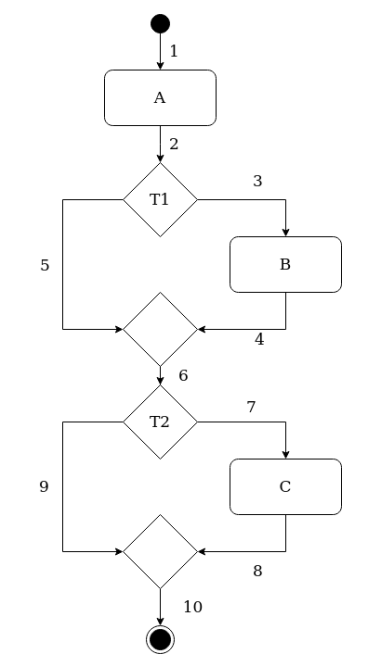
\includegraphics[width=0.3\textwidth]{foto 1.png}
\end{center}
Lo schema proposto raffigura il processo esecutivo di un certo blocco di codice posto all'interno del sistema software, il quale è stato rimpiazzato mediante alcune notazioni grafiche per rendere al meglio la visualizzazione di un percorso. Dal \textit{flow chart} presentato, si articolano un totale di sette percorsi distinti, raggruppati in tre insiemi differenti, inerenti alle descrizioni di \textit{coverage} precedenti. Esempi di quanto detto sono:
\begin{itemize}[label={-}]
    \item \textit{Code coverage} 
    \begin{itemize}
        \item 1;A;2;3;B;4;6;7;C;8;10 
    \end{itemize}
    \item \textit{Branch coverage} 
    \begin{itemize}
        \item 1;A;2;3;B;4;6;7;C;8;10
        \item 1;A;2;5;6;9;10
    \end{itemize}
    \item \textit{Path coverage}
    \begin{itemize}
        \item 1;A;2;3;B;4;6;7;C;8;10
        \item 1;A;2;5;6;9;10
        \item 1;A;2;5;6;7;C;8;10
        \item 1;A;2;5;6;9;10
    \end{itemize}                            
\end{itemize}
\textit{Path coverage} è sicuramente il meccanismo più dispendioso dei tre, e data la complessità che lo caratterizza si riserva solamente per punti critici, anche se questo comporta, da canto suo, ad un elevato dispendio in termini di mantenimento e stesura del codice. 

\subsection*{Black vs White}
\large
\textit{Black-box} e \textit{white-box} differiscono principalmente sull'approccio adoperato per garantire il giusto livello di confidenzialità, il primo incline al risultato tangibile mentre il secondo affine alla bontà della struttura interna del sistema software. In relazione a quale delle due risulti migliore non è possibile rispondere, poichè sono caratterizzate entrambe da imperfezioni e priviliegi. Perciò sono illustrate le peculiarità di ognuno dei meccanismi.
\begin{itemize}[label={ }]
    \item \textit{Black-box testing}
    \begin{itemize}
        \item \textit{Pro}\\\textit{Black-box testing} si fonda solo sul \textit{comportamento} della soluzione software attuata, in cui non è imposta la comprensione del \textit{code base} ma di approcciare un giusto livello di logica algoritmica affinchè si possa riconoscere il \textit{behavior} atteso. Spesso i test sono implementati in modo da riflettere i soli requisiti funzionali, da cui risulterà immediata la comprensione di quale funzionalità non eroghi correttamente l'\textit{output} desiderato, solo se adoperata la corretta struttura di \textit{isolamento} tra entità del sistema software.
        \item \textit{Cons}\\Data la costruzione di un insieme di \textit{test} legati al \textit{comportamento} atteso non è garantito un ottimo livello di copertura, a causa del livello alto di analisi imposto dall'approccio \textit{black-box}.
    \end{itemize}
    \item \textit{White-box testing}
    \begin{itemize}[label={-}]
        \item \textit{Pro}\\Approcci correlati al metodo \textit{white-box} garantiscono l'instaurazione di un elevato livello di \textit{confidenzialità}, poichè stabiliscono la costruzione di test sull'architettura del \textit{code base}, da cui deriva la necessità di studiare e comprendere le particolarità della soluzione sviluppata.
        \item \textit{Cons}\\Nonostante esprima un \textit{coverage} estremamente ampio, comporta ad un numero crescente di percorsi possibili, i quali possono aumentare in maniera smisurata e, pertanto, provocare un grande dispendio di risorse. Il codice per un test simile è piuttosto difficile da implementare e da mantenere.
    \end{itemize}
\end{itemize}

\subsection*{Test the tests}
\large
La bontà di un \textit{test} è la correttezza in cui sia possibile analizzare e rilevare \textit{difetti} che si possano tradurre in \textit{malfunzionamenti} all'interno del \textit{software system}. Tuttavia, la difficoltà principale consiste nella valutazione dei test sviluppati in maniera tale da osservare il grado di validità correlato.\vspace*{14pt}\\
L'effettività desiderata da un qualsiasi team di sviluppo prevede la realizzazione di test di pregievole qualità in grado di elencare tutti gli aspetti errati del sistema software; ma come è possbile stabilire se un codice di verifica sia ben strutturato?\vspace*{14pt}\\
Ciò avviene tramite la creazione di \textit{mutanti}, ossia versioni del \textit{code base} che contengono \textit{errori} e \textit{difetti}, affinchè si possano poi tradurre in \textit{malfunzionamenti}. Ottenuto in \textit{input} il \textit{mutant}, il \textit{software testing} ideato dovrebbe individuare i \textit{bug} e renderli visualizzabili ad attori esterni, garantendo in questo modo codici di verifica corretti. Nel caso opposto questo potrebbe segnalare equivoci effettuati all'interno della soluzione.

\subsection*{Isolamento}
\large
Gli approcci descritti fino ad ora possono essere adoperati con tre modalità di precisione, in cui il più utilizzato appartiene a \textit{unit testing}. Dato che opera su singola unità, come classi e metodi, si fonda sul concetto di \textit{isolamento}.\vspace*{14pt}\\
In relazione alla comprensione del concetto di \textit{isolation} è bene soffermarsi su tre azioni sequenziali che potrebbero caratterizzare un comune processo di verifica:
\begin{itemize}[label={-}]
    \itemsep0em
    \item Avviene l'instanzazione dell'oggetto
    \item Si opera sull'oggetto affinchè sia manipolabile
    \item Si attuano funzionalità di verifica dello stato dell'oggetto dopo aver richiamato il metodo interessato
\end{itemize}
Nonostante spesso test del genere possano essere adeguati per analizzare la validità della soluzione software, non sempre sono in grado di indicare se \textit{malfunzionamenti} siano imputabili sull'istanza in questione oppure a logiche interne; si ricorda la figura della dipendenza, in cui una classe software può richiamare funzionalità di altri elementi del modello per elaborare comportamenti interni. Rispetto a quando proposto occorre un \textbf{meccanismo di isolamento}.\vspace*{14pt}\\
L'implementazione di una tecnica simile avviene tramite l'impiego di \textit{controfigure}, le quali forniscono automaticamente i parametri necessari a classi analizzate e devono essere sviluppate tramite una minima logica algoritmica, in modo tale che effettività errate non siano associabili alle nuove entità introdotte.\vspace*{14pt}\\
\textit{Caso di studio}\\
\begin{center}
    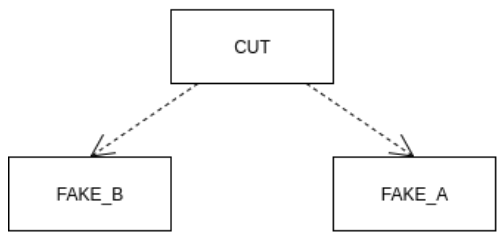
\includegraphics[width=0.4\textwidth]{foto 2.png}
\end{center} 
Nell'esempio proposto si osservano le due entità \textit{FakeA} e \textit{FakeB}, le quali rappresentano le controfigure delle classi concrete che riportano i dati necessari per inizializzare le fasi di test. Tuttavia, essendo elementi del modello legati a logica algoritmica, l'assenza di un livello di astrazione potrebbe disorientare le fasi di verifica attuate.\vspace*{14pt}\\
La soluzione prevede l'inserimento di interfacce, poste tra classe verificata e dipendenze della singola unità modellativa, poichè in totale assenza non sarebbe possibile associare l'errore riscontrato. Concludendo, occorre che anche codici dei test siano relativi a un layer minimo di qualità, dato che contribuiscono ad un maggiore isolamento dei termini e su cui è possibile, conseguentemente, adeguare \textit{pattern} di differente natura.
\begin{center}
    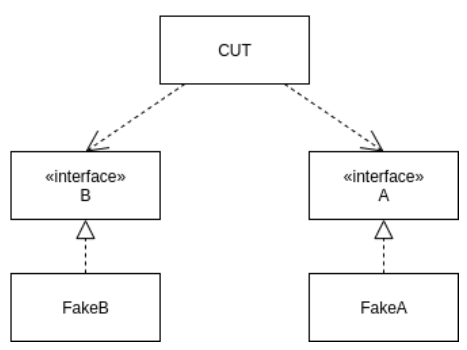
\includegraphics[width=0.4\textwidth]{foto 3.png}
\end{center} 
\end{document}